\documentclass{article}

\usepackage{tikz}
\usepackage{amsmath}
\usepackage{framed}
\usepackage{hyperref}
\usepackage{caption}
\usepackage{subcaption}
\usepackage{wrapfig}
\usepackage{float}

\newcommand{\iidist}{\stackrel{iid}{\sim}}
\newcommand{\mse}{\ensuremath{\text{MSE}}}
\newcommand{\sse}{\ensuremath{\text{SSE}}}
\newcommand{\figref}[1]{Figure \ref{#1}.}

\begin{document}

\section{Introdution and Motivation}
\textcolor{red}{\Large LIA Put your introduction here.}

\section{The Model}
We model the absorption via the following cascading compartmental decay model.

\tikzset{
  compartment/.style={
    rectangle, 
    minimum size=15mm, 
    thick, 
    draw=black!50
  }
}
\begin{center}
\usetikzlibrary{positioning,fit}
\begin{tikzpicture} [node distance=10mm and 20mm,
		    ]
\node (Xa) [compartment]	     {$X_a$};
\node (X)  [compartment,right=of Xa] {$X$};
\node (exitx) [right=of X] {};
\draw[-latex] (Xa) -- node[above] {$k_a X_a$} (X);
\draw[-latex] (X)  -- node[above] {$K X$} (exitx);
\end{tikzpicture}
\end{center}

The initial amounts are given by $X_a(0) = F X_0$ and $X(0) = 0$, where $F$ is the fraction of the drug absorbed by the mouse and $X_0$ is the amount administered.  So, we have the following system of differential equations
  \begin{align*}
    \frac{dX_a}{dt} &= -k_a X_a(t),\\
    \frac{dX}{dt}   &= k_a X_a(t) - KX(t),\\
     X_a(0) &= F X_0 , \quad X(0) = 0.
  \end{align*}

We wish to estimate $F$, the fraction of drug absorbed, $k_a$ the rate of absorption into the blood, and $K$ the rate of dispersion from the blood.

The data recorded are in terms of concentration of the drug in the cell, if $V$ is the average volume of the cell, is introduced and then we can reparameterize $X$, $C(t) = X(t) / V$, and the parameter. 

Note that this system can be solved analytically, as it is linear,
$$
  \frac{d}{dt}
  \begin{pmatrix}
  X_a \\
  X
  \end{pmatrix}
  =
  \begin{pmatrix}
    -k_a & 0 \\
    k_a  & -K
  \end{pmatrix}
  \begin{pmatrix}
  X_a\\
  X
  \end{pmatrix}, \quad \begin{pmatrix} X_a(0) \\ X(0) \end{pmatrix} = \begin{pmatrix} FX_0 \\ 0\end{pmatrix}.
$$ 

The solution for the absorption into the blood is given by 
\begin{align*}
X_a(t) &= FX_0 \big( k_ae^{-k_at} \big),\\ 
X(t) &= \frac{k_a F X_0}{k_a - K}\big( e^{-Kt} - e^{-k_a t}\big).
\end{align*}

\section{Methods}

\subsection{Model Fit}
We must first fit the model. Initially, one might fit the scaled solution (i.e. concentration) 
$$C(t) = \frac{X(t)}{V} = \frac{F}{V} \cdot X_0 \cdot \frac{k_a}{k_a -K}\big( e^{-Kt} - e^{-k_a t}\big).$$
However the factor $k_a - K$ in the denominator makes this optimization step unstable.  Instead we optimize the system of differential equations, with the added scaling factor $1 / V$ to $X$.  We fit the parameters of the model by optimizing the function that returns a numerical solution to the differential equation  by optimizing the squared error fit of the data.  Note that each mouse has a different initial dosage (to maintain the assumption of constant kinetic parameters across groups), hence we pool the error from 10 separate fits.  That is the pooled SSE within groups is given by:
  $$
    SSE = \sum_{i=1}^{10} \sum_{j=1}^4 \big(C(t_j,y_{0i}|\hat k_a,\hat K,\widehat{F/V},) - Cobs_{i,j}\big)^2,
  $$
  Where the $i$ indexes over the mice and $j$ indexes time.  Note $\hat k_a,\hat K,\widehat{F/V}$ are independent of each.  Our fitting goal is to minimize this quantity with respect to the parameters $F/V,k_a,$ and $K$.  

\subsection{MCMC Parameter Estimate Distributions}  

We use Markov Chain Monte Carlo methods to obtain parameter estimate distributions.  In particular, we adapt codes written by Haario \cite{hario} implementing adaptive Metropolis MCMC parameter estimates.  Initially, our algorithm calculated the pooled SSE via numerical solutions to the ODE which has computationally prohibitive in \texttt{MatLab}.  We modified the calculation of the SSE in the MCMC step to use the exact solution as the stability difficulties in the optimization are no longer relevant. 

\subsection{Inference}

Finally, we conduct statistical inference on the parameter distributions obtained on each mouse group to identify any kinetic differences.  This is accomplished by merely forming distributions of the \emph{differences} of the parameters between each group and forming 95\% confidence intervals and observing if 0 is captured within them.  We form these intervals from the MCMC chains, and a subset of the chains to observe any effects of auto-correlation.

Codes carrying out this procedure can be obtained at \url{https://github.com/kjoyce/math445_project}.
  
\section{Results} 
\textcolor{red}{\Large DEREK AND LIA
Two Things -- When you compile, you may have to compile twice for the figure refs to be created... Or just make sure you also download write\_up.aux, write\_up.log, and write\_up.out and keep the filename write\_up.tex. Please ask if there are tex questions, or I can just compile them if it is a headache, Lia.  Second, I adjusted for autocorrelation as Leonid had suggested.  It amounted to just taking every 10th element in the chains.  I have explained the last bit so don't worry about it, Derek.
}

\begin{figure}[H]
  \begin{subfigure}[b]{.45\textwidth}
    \includegraphics[width=\textwidth]{group_a_plotmatrix.pdf}
    \caption{Model fits for Mice A.}
    \label{fits:a}
  \end{subfigure}
  \begin{subfigure}[b]{.45\textwidth}
    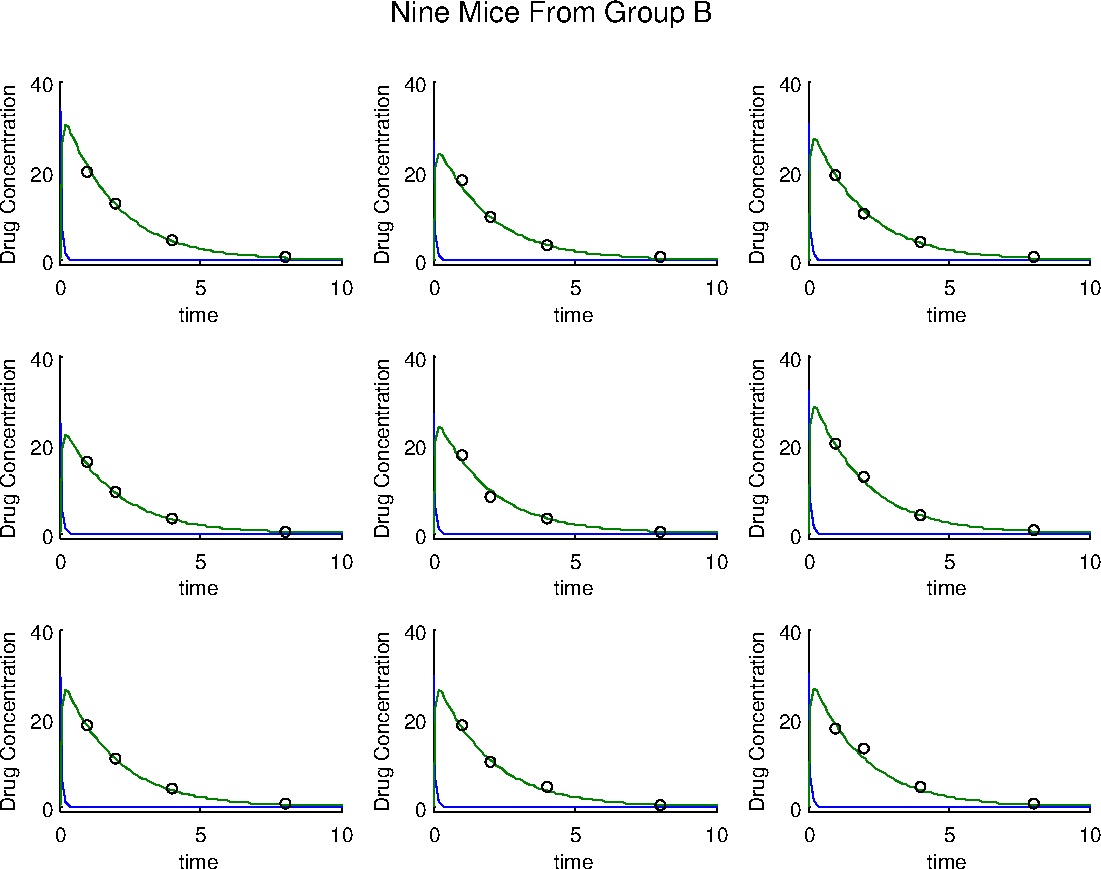
\includegraphics[width=\textwidth]{group_b_plotmatrix.pdf}
    \caption{Model fits for Mice B.}
    \label{fits:a}
  \end{subfigure}
  \caption{Model fits for each group.}
  \label{fits}
\end{figure}
EXPLAIN \figref{fits} HERE

\begin{figure}[H]
  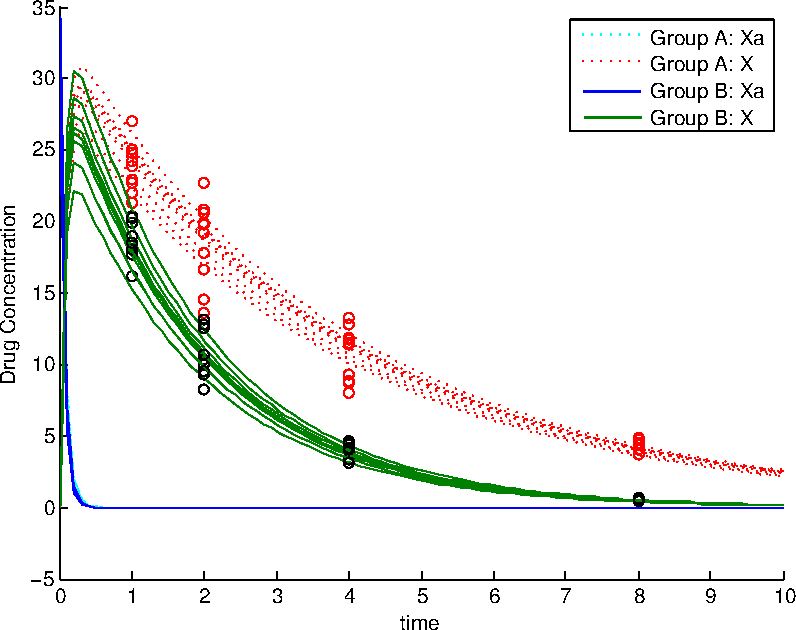
\includegraphics[width=\textwidth]{all_fitted.pdf}
  \caption{All model fits.}
  \label{allfit}
\end{figure}
EXPLAIN \figref{allfit} HERE

\begin{figure}[H]
  \begin{subfigure}[t]{.45\textwidth}
    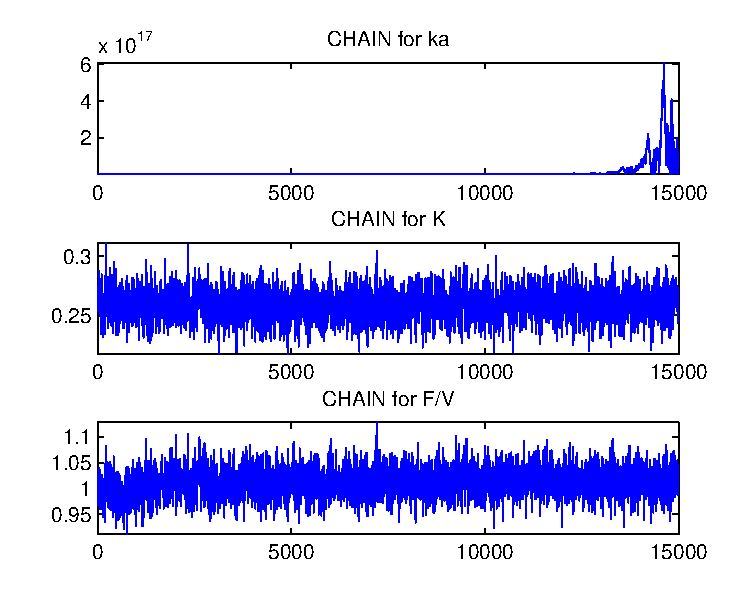
\includegraphics[width=.85\textwidth]{mice_a_chains.pdf} 
    \caption{Chains for Mice A.}
    \label{amcmc:chain}
  \end{subfigure}
  \begin{subfigure}[t]{.45\textwidth}
    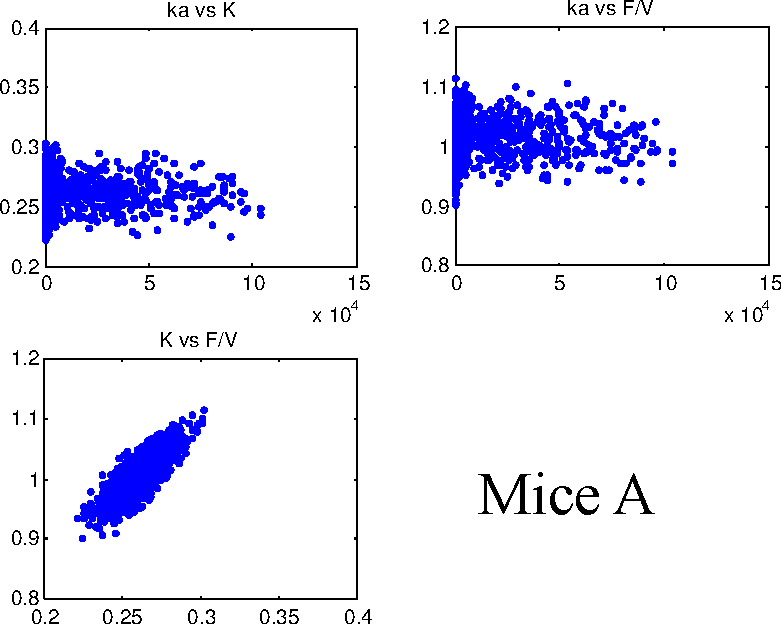
\includegraphics[width=\textwidth]{mice_a_joint_dists.pdf}
    \caption{Joint distributions for Mice A.}
    \label{amcmc:dists}
  \end{subfigure}
  \caption{MCMC runs for Mice A.}
  \label{amcmc}
\end{figure}

\begin{figure}[H]
  \begin{subfigure}[t]{.45\textwidth}
    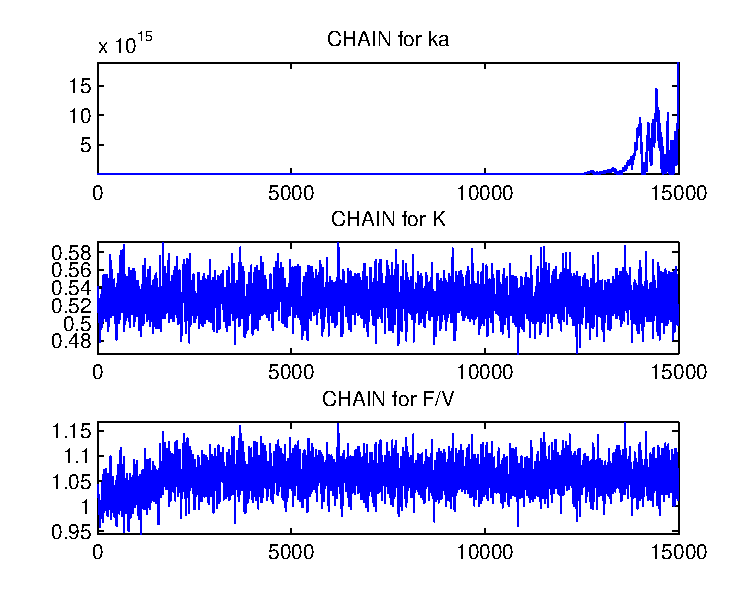
\includegraphics[width=.85\textwidth]{mice_b_chains.pdf} 
    \caption{Chains for Mice B.}
    \label{bmcmc:chain}
  \end{subfigure}
  \begin{subfigure}[t]{.45\textwidth}
    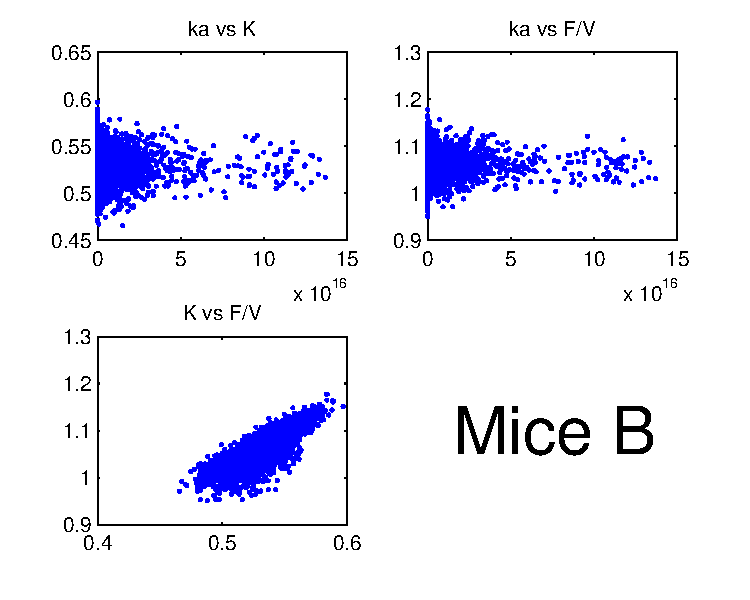
\includegraphics[width=\textwidth]{mice_b_joint_dists.pdf}
    \caption{Joint distributions for Mice B.}
    \label{bmcmc:dists}
  \end{subfigure}
  \caption{MCMC runs for Mice B.}
  \label{bmcmc}
\end{figure}

Explain both \figref{amcmc} and \figref{bmcmc} here.  You can reference subfigures \figref{amcmc:chain} and \figref{bmcmc:dists}.

\begin{figure}[H]
  \begin{subfigure}[b]{.45\textwidth}
    \includegraphics[width=\textwidth]{drug_abs_diff.pdf} 
    \caption{Distribution for difference in $F/V$, fraction of absorption. \\
    The 95\% CI:$[-0.1243,0.0292].$}
     
    \label{absorp}
  \end{subfigure}
  \begin{subfigure}[b]{.45\textwidth}
    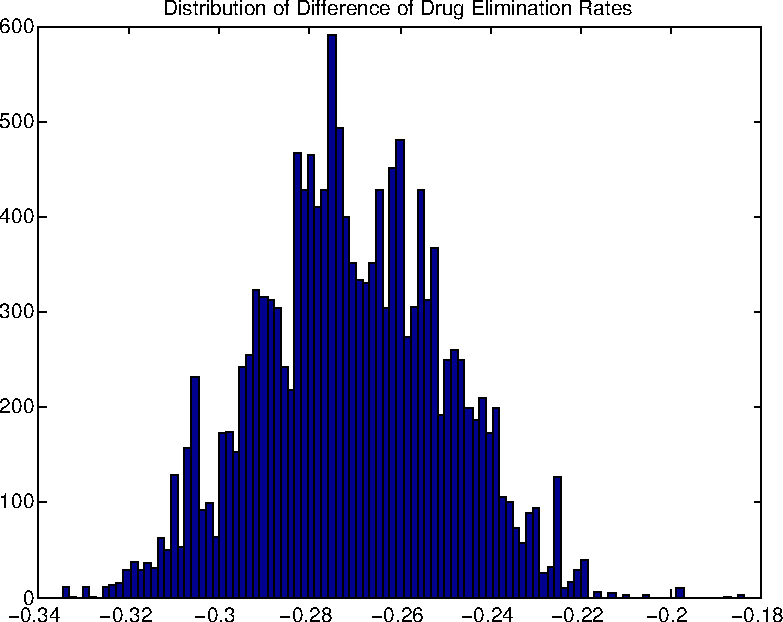
\includegraphics[width=\textwidth]{elim_rate_diff.pdf}
    \caption{Distribution for difference in $K$, elimination rate constant.\\
    The 95\% CI: $[-0.3114,   -0.2278].$}
      
    \label{elim}
  \end{subfigure}
  \caption{ Parameter estimate distributions. }

\end{figure}

EXPLAIN \figref{absorp} and \figref{elim}

\begin{figure}[H]
  \begin{subfigure}[b]{.45\textwidth}
    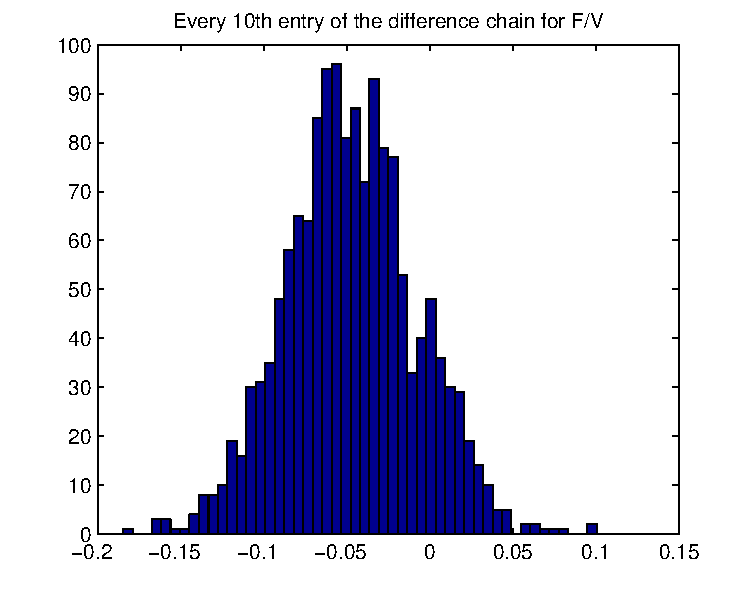
\includegraphics[width=\textwidth]{auto_cor_FV.pdf}
    \caption{Distribution for difference in $F/V$, autocorrelation corrected. \\
    The 95\% CI:$ [-0.1228,0.0284]$.}
     
    \label{autoabsorp}
  \end{subfigure}
  \begin{subfigure}[b]{.45\textwidth}
    \includegraphics[width=\textwidth]{auto_cor_K.pdf}
    \caption{Distribution for difference in $K$, autocorrelation corrected.\\
    The 95\% CI: $[-0.3107,-0.2278]$.}
    
    \label{autoelim}
  \end{subfigure}
\caption{ Every 10th chain element removed correcting for autocorrelation. }
\label{autocor}
\end{figure}

\figref{autocor} displays the results of adjusting for auto-correlation. We have selected every 10th element of the distribution chain to correct for correlation between successive elements in the Markov process.  Due to the size of the chain, however, the effects of this autocorrelation are negligable as can be seen from the above results.

\begin{thebibliography}{[99]}
\bibitem{hario} Haario H., MCMC for (Biological) Modeling, Lappeentranta University of Technology, Finland. 2012
\bibitem{notes} Graham J. and Kalachev L.  Lecture Notes for Statistical, Dynamical, and Computational Modeling. University of Montana. 2012.
\end{thebibliography}
\end{document}

